\section{Visitor}

O padrão Visitor define uma estrutura que permite implementar 
operações em um objeto ou em uma coleção de objetos sem 
alterar sua implementação. Para isso, é definida uma classe 
abstrata que define as operações que o Visitor deve implementar 
para cada tipo de elemento da coleção. Dessa forma, cada 
objeto da coleção implementa apenas uma operação, que recebe 
um Visitor genérico e realiza a operação desejada sem 
conhecê-la.

Esse padrão permite estender objetos para novas operações 
sem comprometer sua implementação ou poluir as classes com 
diversas operações que não são de sua responsabilidade. Ele 
também permite que operações diferentes sejam executadas 
dependentes da implementação do objeto. Por exemplo, em uma 
coleção de objetos do tipo da interface A que é implementada 
por objetos do tipo B e C, um Visitor pode realizar uma 
operação diferente se o objeto for do tipo B ou do tipo C.

\begin{figure}[htb]
	\caption{\label{visitor_struct}Estrutura do Visitor}
	\begin{center}
	    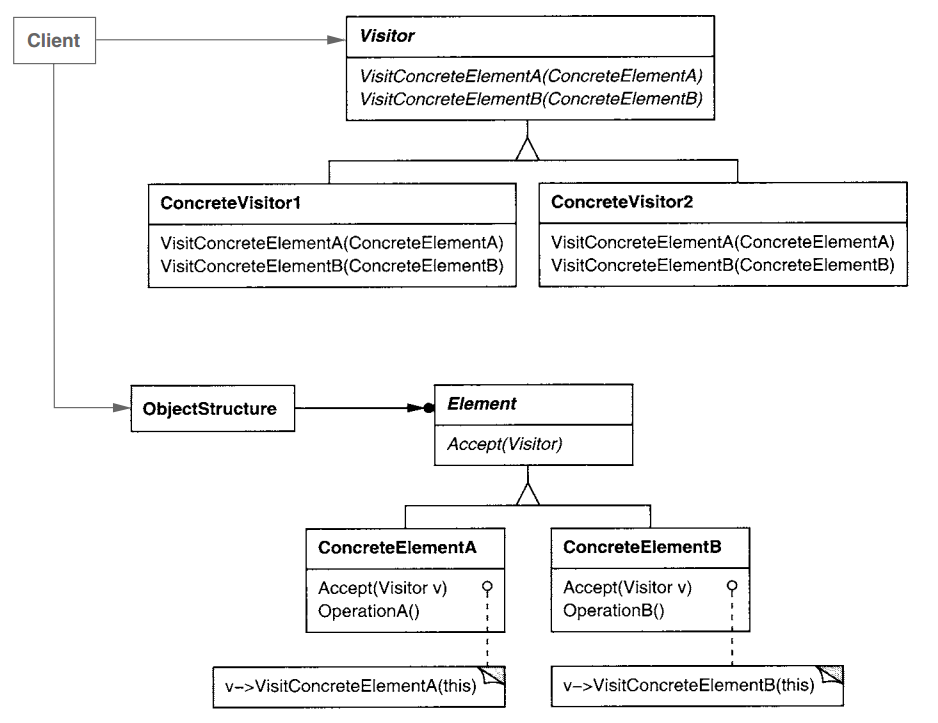
\includegraphics[scale=0.3]{5_padroes-contexto-funcional/5.3_comportamentais/5.3.11_visitor/diagram.png}
	\end{center}
\end{figure}

\subsection*{Exemplo Orientado a Objetos}

\begin{figure}[htb]
	\caption{\label{visitor_exemplo1}Exemplo de Visitor}
	\begin{center}
	    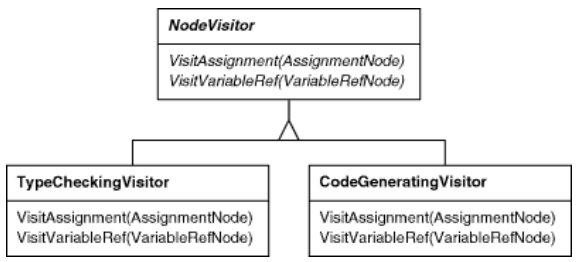
\includegraphics[scale=0.3]{5_padroes-contexto-funcional/5.3_comportamentais/5.3.11_visitor/visitor_exemplo1.png}
	\end{center}
\end{figure}

\begin{figure}[htb]
	\caption{\label{visitor_exemplo2}Exemplo de Estrutura Visitada}
	\begin{center}
	    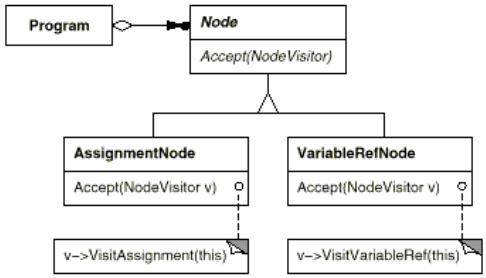
\includegraphics[scale=0.3]{5_padroes-contexto-funcional/5.3_comportamentais/5.3.11_visitor/visitor_exemplo2.png}
	\end{center}
\end{figure}

\begin{lstlisting}[caption={Visitor Orientação a Objetos},label=oovisitor]



\end{lstlisting}

\subsection*{Contexto Funcional}

\begin{comment}
O Visitor é mais um caso em que funções de alta ordem ajudam a 
economizar novas classes e interfaces. Basta definir uma função 
que receba como parâmetro um valor do tipo encapsulado pela 
coleção e retornar um valor do mesmo tipo com a operação 
realizada. Funções do tipo map, que podem ser usadas para 
realizar uma operação em uma coleção, contribuem para essa 
implementação.

Porém, a funcionalidade do Visitor que permite realizar 
operações diferentes dependendo da implementação do objeto 
também é interessante e pode ser alcançada utilizando 
pattern matching. [terminar esse texto]
\end{comment}

\begin{lstlisting}[caption={Visitor Funcional},label=fpvisitor]
    

    
\end{lstlisting}